\documentclass[a4paper,11pt]{article}
\usepackage[utf8]{inputenc}
\usepackage[T1]{fontenc}
\usepackage[a4paper,top=1in, bottom=1in, left=1in, right=1in]{geometry}
\usepackage[french,magyar]{babel}
\def\magyarOptions{defaults=prettiest}

\usepackage[none]{hyphenat}
\usepackage{amsfonts,amsmath,amssymb}
\usepackage{fancyhdr}
\usepackage[none]{hyphenat}

\usepackage{hyperref}
\hypersetup{
    colorlinks=true,
    linkcolor=black,
    filecolor=magenta,      
    urlcolor=blue,
}
\usepackage{float}
\usepackage[dvipsnames]{xcolor}
\usepackage[nottoc,notlot,notlof]{tocbibind}
\usepackage{graphicx}
\usepackage{caption}
\usepackage{subfig}
\usepackage{enumitem}
\usepackage{booktabs}
\usepackage[export]{adjustbox}
\usepackage{enumitem}
\setlist[1]{itemsep=-5pt}
\pagestyle{fancy}
\fancyhead{}
%\fancyfoot{}
\renewcommand{\headrulewidth}{0pt}

\usepackage{hyperref}

\usepackage{listings}
 
\urlstyle{same}

%\renewcommand{\baselinestretch}{1.5}

\begin{document}
%\emergencystretch 3em
\sloppy

\begin{titlepage}
\begin{center}
%\vspace{1cm}
\begin{figure}[t!]
	\begin{center}
	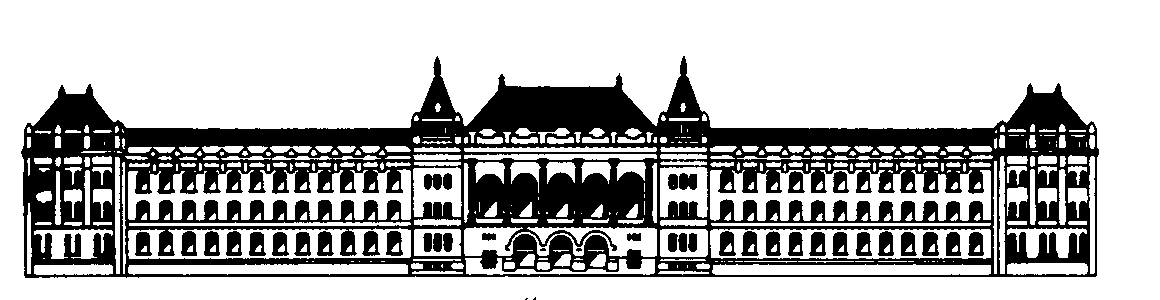
\includegraphics[scale=0.2]{bme.png}
	\label{a:bme}
	\end{center}
\end{figure}
\textbf{{Budapesti Műszaki és Gazdaságtudományi Egyetem}}\\
Villamosmérnöki és Informatikai Kar\\
Méréstechnika és Információs Rendszerek Tanszék\\
\vfill
\huge\textbf{{Rendszerarchitektúrák}}\\[3mm]
\Large{Házi feladat}\\[3mm]
\Large\textbf{{AXI - SPI perifériaillesztő}}\\
\vfill
\Large{Kardos Bálint, ZI84PX}\\
\Large{Murányi Péter, A74MW9}\\
\Large{Konzulens: Raikovich Tamás}\\
\vfill
\today \\

\end{center}
\end{titlepage}

\tableofcontents
\thispagestyle{empty}
\clearpage
\setlength{\parindent}{0em}
\setlength{\parskip}{1em}

\setcounter{page}{1}
\setcounter{tocdepth}{4}
\setcounter{secnumdepth}{4}


\section{Feladat}
A félév során egy SPI Master periféria Verilog nyelven történő fejlesztése volt a feladat, amely egy AXI Lite perifériabusz vezérlőre került illesztésre. Az így elkészített rendszer működőképessége szimulációval került ellenőrzésre. Szimulációban a perifériabusz vezérlését BFM valósítja meg, ami úgy tesz, mintha AXI Lite Master lenne az AXI Lite időzítési kritériumait figyelembe véve. Az SPI Masterre egy Microchip által fejlesztett EEPROM Verilog modul csatlakozik. A szimuláció az EEPROM-ba történő írást és ennek a beírt adatnak a visszaolvasását valósítja meg.
\begin{figure}[H]
	\begin{center}
	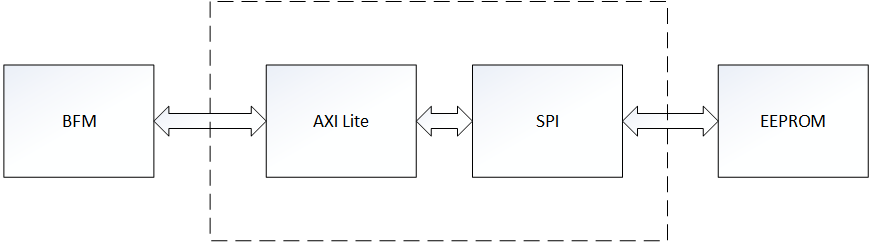
\includegraphics[scale=0.7]{genbd.png}
	\caption{A kitűzött feladat blokkdiagramja}
	\label{fig:genbd}
	\end{center}
\end{figure}

\section{AXI Lite}

\section{SPI - Serial Peripheral Interface Bus}
A Serial Peripheral Interface busz egy szinkron soros interfész, amely elsősorban beágyazott rendszerekben fordul elő, ahol az egymással kommunikálni kívánó eszközök közötti távolság rövid. Az SPI interfész shift regisztereken alapul. A kommunikáció master-slave jellegű, ahol a master vezérli a kommunikációt: szolgáltatja az órajelet, valamint egy külön vezetékkel engedélyezi a hozzákapcsolt slave perifériákat.\\
Ennek az a hátránya, hogy minden slave perifériához külön kiválasztó vezetéket kell használni. A szükséges I/O lábak csökkentése érdekében használhatunk dekódert. 
Az SPI busz jelvezetékei:
\begin{itemize}
	\item SCLK: órajel, amit a master biztosít,
	\item MOSI: a master eszköz soros adatkimenete, amely a slave soros adatbemenetére csatlakozik,
	\item MISO: a master eszköz soros adatbemenete, amely a slave soros adatkimenetére csatlakozik,
	\item $\overline{CS}$n: slave eszköz kiválasztó jele, ahol n az n-edik eszközhöz tartózó engedélyező jele.
\end{itemize}
A kommunikáció megkezdéséhez a master biztosítja az órajelet és logikai 0-ba állítja a megfelelő $\overline{CS}$n slave kiválasztó jelét. A kommunikáció egyszerre kétirányú - vagyis míg a léptetőregiszter bemenetén sorosan fogadja a biteket ugyanakkor a regiszter másik végén kiléptetjük annak előző tartalmát. Ezért például 16 órajellel a master és slave 16 bites shift regisztereinek a tartalma helyet cserél. Az SPI periféria fontos tulajdonsága az órajel élének és polaritásának megválasztása.
\begin{figure}[H]
	\begin{center}
	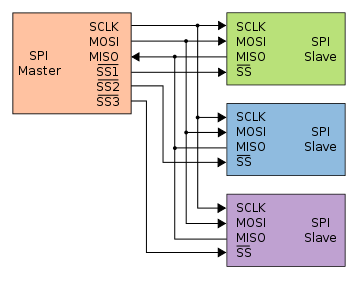
\includegraphics[scale=0.7]{SPI_three_slaves.png}
	\caption{SPI busz: 1 master és 3 független slave eszköz}
	\label{fig:SPI_three_slaves}
	\end{center}
\end{figure}
\begin{figure}[H]
	\begin{center}
	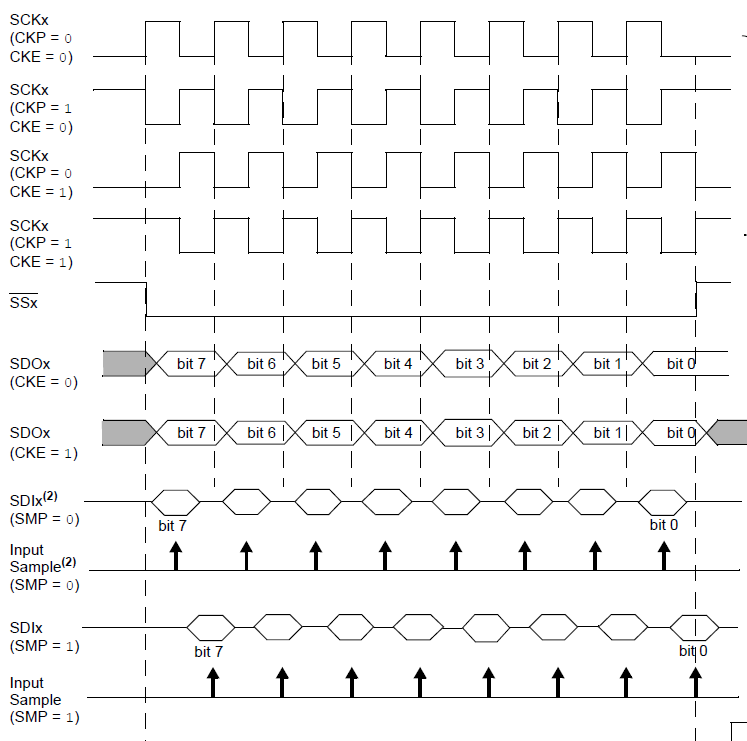
\includegraphics[scale=2]{spi_clkdiag.png}
	\caption{Az SPI periféria órakonfigurációs beállításai}
	\label{fig:spi_clkdiag}
	\end{center}
\end{figure}

\section{Tervezés}

blablabla

\begin{figure}[H]
	\begin{center}
	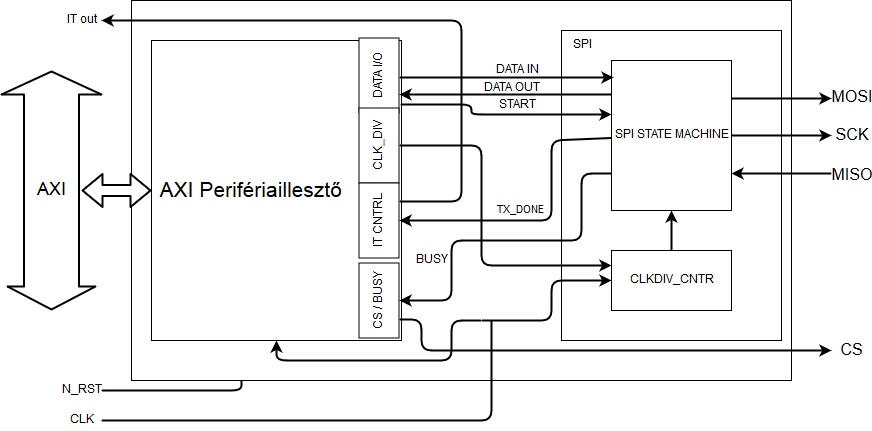
\includegraphics[scale=0.5]{system_blockdesign.png}
	\label{fig:system_main}
	\end{center}
	\caption{Az eszköz blokkdiagramja}
\end{figure}

\begin{figure}[H]
	\begin{center}
	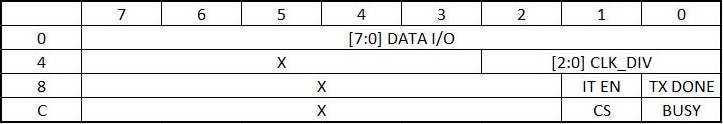
\includegraphics[scale=1]{reg_set.JPG}
	\label{fig:registers}
	\end{center}
	\caption{A periféria regiszterei}
\end{figure}

\section{Verilog megvalósítás}

\subsection{AXI Lite illesztő}
Az AXI lite illesztő a Xilinx saját példája alapján lett megírva. Minden csatorna elkülöníthető, a funkciójukat önállóan valósítják meg. Mivel általában az ehhez hasonló rendszerek active-low reset-et használnak, így itt is ez lett alkalmazva. A reset és órajel vonalak minden egységhez csatlakoznak, a reset a rendszer minden elemét egy megadott indítási állapotba hozza.

Mivel regisztereket nem szabad egyszerre több helyről is írni, ezért a bemeneti és kimeneti regisztereket el kell különíteni az AXI illesztőn belül. Egyes regiszterek értékét csak az AXI master változtatja, ezeket egyszerűen vissza lehet kötni a kimeneti regiszterekbe, viszont egy csomó regiszter más értéket ad ki olvasáskor, mint amit beleírtunk, ezeknek a kezelésére külön logika szükséges.

Az írási csatornát kezelő logika végzi a bejövő adatok kezelését. Érvényes AWVALID jelre, ha éppen nem folyik írás, jelez az AWREADY vonalon hogy képes érvényes cím fogadására és mintavételezi a AWADDR csatornát. Ezután ugyanez a handshake folyamat megy végbe az írási adat csatornán is. Ha mindkét csatornán érvényes volt a tranzakció, megtörténik a tényleges írás a címzett adatregiszter AXI\textunderscore WSTRB által megadott megfelelő bájt vonalaiba. Ezzel együtt történik az írás válasz generálása a saját csatornáján, ami itt mindig nulla: írás OK. Mivel az eszköz úgy lett megtervezve hogy az adat I/O regiszterbe való írás indít egy új SPI tranzakciót, így szükség van arra hogy detektáljuk mikor történik írás a regiszterbe. Erre egy külön regiszter lett létrehozva ami 1-be állítódik amikor az AXI Lite nullás regiszterébe történik írás, 0-ba ha bármi más történik. Ezzel egy egy órajelű start jelet tudunk létrehozni amit az SPI modulnak továbbítva megtörténhet az írás.

Az olvasási csatorna végzi a master felől jövő írási kérések kiszolgálását. Az olvasás mindössze két csatornát igényel. Érvényes olvasási handshake után a mintavételezett címnek megfelelő regiszterből megtörténik az adat kiírása az olvasási válasz státusszal (itt mindig nulla) együtt. A kimenő regiszterek rendre mind wire adattípust használnak, ezek meghajtása vagy egy belső regiszterről történik, aminek az értékét valamilyen logika határozza meg, vagy fixen nullára vannak bekötve (mivel 32 bitesek az AXI Lite regiszterek, míg legfeljebb is csak 8 bit van meghajtva egy regiszterben).

A regiszterek funkciójuktól függően különbözően viselkednek. Az I/O regiszter írási oldalról az SPI adatbemenetére kapcsolódik, míg olvasási oldalról az adatkimenetéhez van kötve. Ennek a regiszternek az írása egyben egy új SPI kommunikációt is elindít. Az órajelosztást állító regiszter a beírt értékét adja vissza olvasáskor, illetve közvetlenül csatlakozik az SPI clkdiv bemenetéhez. Az ITENABLE és TXDONE biteket tartalmazó regiszter ennél összetettebben működik. A TXDONE bit minden írás befejeződésekor magas állapotba kerül. Innen nullázható egy 1-es beírásával, illetve egy új SPI ciklus indításával, ami automatikusan nullázza ezt az értéket. A negyedik regiszter a busy és $\overline{CS}$ -t vezérlő biteket tartalmazza, előbbi csak olvasható, utóbbi írható és olvasható is.

Ezeken túl itt van elhelyezve az SPI-t indító logika, illetve a megszakítás generálása. Az SPI indítása egy egyszerű logikai ÉS kapcsolat, ami az I/O regiszterbe történő írást jelző bitet, az SPI használatát jelölő "busy" bit negáltját és CS bit állását fogja össze. Ebből egy egy órajeles start impulzus jön létre ami elindítja az SPI modult. Az interrupt jel hasonló módon, adott bitek megfelelő állása esetén generálódik. Figyelembe veszi, hogy aktiváltuk e az SPI TX\textunderscore ENABLE bitjét, és az SPI modul TXDONE kimeneti bitjét figyeli. Ha ez a kettő egyszerre igaz, egy egy órajeles megszakítást generál, jelölve, hogy befejeződött az SPI kommunikáció.

\subsection{SPI modul}

Az SPI modul két részből áll. Egy órajel osztó számlálóból, illetve az SPI-t vezérlő állapotgépből. Az órajelosztó számláló egy egyszerű 8-bites számláló, aminek a CLKDIV által megadott bitjét csatoljuk ki az SCK órajel megadásához. Ez a jel lesz egyben a kimeneti SCK órajel, illetve ezt használja az állapotgép az adat küldés ütemezésére. A számláló nem szabadonfutó, csak SPI kommunikáció indításakor indul el, addig reset állapotban vár, aminek következményében a kimenete, így SCK nulla lesz.

\begin{figure}[H]
	\begin{center}
	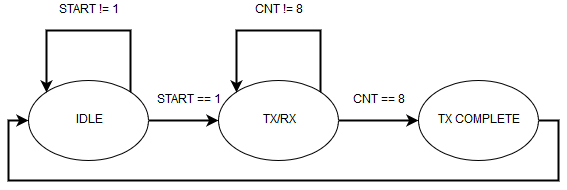
\includegraphics[scale=0.6]{spi_statemachine.png}
	\caption{SPI állapotgépe}
	\label{fig:spistatemchn}
	\end{center}
\end{figure}


Az SPI ciklust egy állapotgép kezeli. Induláskor az IDLE, várakozó állapotban van. Ebben az állapotban a kimeneteket nullázva egy START jelre várakozik. Ha ezt a jelet megkapja,a BUSY jelzőbitet magasra húzza, beolvassa a bemeneti adatot és egy shift regiszterbe menti melynek az MSB-je a MOSI kimenetre van kötve, majd az állapotváltozót megváltoztatva a TX/RX állapotba kerül. Ebben az állapotban az órajelosztó számlálóból kapott jelet figyeli. Mivel minden a főórajel felfutó élére történik, így külön logika kell amivel ellenőrizzük hogy a leosztott órajel felfutó vagy lefutó élen van-e. Ezt egy átmeneti tárolóval oldottuk meg. Ezt minden ciklusban frissítjük a leosztott órajel aktuális állapotával és ezt a két régi és új jelet vizsgáljuk hogy eldöntsük, felfutó vagy lefutó órajele van-e az SCK jelnek. Felfutó élen a MOSI bemeneten lévő adatot egy bemeneti shift-regiszterbe mintavételezzük. Lefutó élen a kimeneti shift regiszter shiftelődik eggyel balra, illetve egy számláló inkrementálódik, ami számolja a kiküldött bitek számát. Ha ennek a számlálónak az értéke eléri a 8-at, tehát az utolsó felfutó él után lefut az SCK az állapotgép a TX COMPLETE állapotba vált. Ebben az állapotban a bejövő shiftregiszter értékét átmásolja az adat kimenetre, továbbá a TXDONE jelet magas értékre húzza. Ebből az állapotból mindig az IDLE állapotba kerül a következő órajelciklusban, ahol a TXDONE és BUSY jelek nullára állnak vissza jelezve hogy új küldésre készen áll.

\section{Szimuláció}
A létrehozott periféria működése szimulációval lett ellenőrizve. A szimulációhoz a Vivado beépített szimulátorát használtuk. A perifériához az AXI interfész felől egy AXI-LITE Master-t szimuláló BFM lett illesztve, míg az SPI oldalról egy Microchip EEPROM funkcionális verilog modellje lett illesztve. A szimuláció egy az EEPROM-ba való írást, majd onnan a beírt adatok kiolvasását valósítja meg.

A szimuláció 100MHz-s órajelet használ, a reset vonal induláskor 20ns ideig aktív alacsony állapotban van, majd visszatér magas szintre, ami elindítja az összes eszközt. Ezek után futnak le az AXI taszkok, amik inicializálják az SPI perifériát, beírnak 3 bájtot az illesztett EEPROM-ba, majd ezeket ugyanonnan kiolvassa. Az egész szimuláció 20us-ot vesz igénybe.

Az SPI modul /16 órejelosztást használ, amivel az SCK 6,25 MHz lesz. A SPI megszakítás küldője be lett kapcsolva ugyanis ezt használjuk az SPI tranzakciós ciklus befejeződésének figyelésére. A $\overline{CS}$ jelet manuálisan állítjuk, az SPI megfelelő regiszterébe való írással.
\subsection{BFM}

A busz funkcionális modell egyszerű verilog taszkokkal lett megvalósítva. Ezek a taszkok az AXI LITE interfészt ismertető részben bemutatott időzítési diagram szerint lettek megírva. A taszkokban az órajel felfutó éle után mindenhol egy 1ns-os késleltetés lett elhelyezve, hogy szimuláljuk a rendszerben a flip-flop-ok set-up és hold késleltetésüket. Az írási taszk két bemenettel rendelkezik, írási cím és írási adat. Az olvasási taszk egy bemenet és egy kimenettel rendelkezik: az olvasandó adat címe és a beolvasott adat. Verilog taszkok kimenetein szimulációban csak a taszk befejeződését követően jelenik meg az új adat, attól függetlenül hogy a taszkban hol történt ténylegesen a kimeneti regiszter írása.

\subsection{EEPROM}
Az eszközhöz egy Microchip 25AA010A EEPROM szimulációs verilog modellje van illesztve, hogy a valós működés is tesztelve legyen. Ez a modul egy 1kbit méretű flash EEPROM-ot valósít meg, valós időzítési értékekkel. Az eszköz leírása \href{http://ww1.microchip.com/downloads/en/DeviceDoc/21832H.pdf}{ezen a linken} érhető el.

Az eszköz valós időzítéseket is szimulál, ezért például az SCK órajel nem lehet gyorsabb 10MHz-nél, ugyanis az eszköz nem lesz képes elég gyorsan reagálni az órajel változására. Ezt az SPI órajelosztójának megfelelő beállításával lehet elérni.

Hogy az eszközt írhassuk, először egy instrukciót kell neki küldeni ami engedélyezi az írást az eszközön belül. Ehhez egy külön írási ciklusra van szükségünk ahol $\overline{CS}$ jelet aktív alacsonyra kell húzni, majd az írásengedélyező (WREN) parancsot kiküldve a $\overline{CS}$ jelet egy órajelciklus idejére vissza kell engedni magas szintre. Ha ezt nem tesszük meg, nem fogunk tudni írni az eszközbe. Ezek után lehet ténylegesen írni az eszközt. Íráskor először egy 8-bites írás instrukciót kell kiküldeni, ez után jöhet a cím, szintén 8-biten, majd ezt követően kezdődik meg a tényleges adat kiküldése. Lehet bájtos, illetve burst módban írni, viszont burst módban maximum 16 bájtot lehet kiküldeni, ugyanis az EEPROM csak ekkora bemeneti bufferrel rendelkezik. Az írást a $\overline{CS}$ magasra húzásával lehet befejezni, ekkor az írásengedélyező belső flag automatikusan 0-ra áll vissza. Az EEPROM verilog modelljében apró változtatásokat kellett eszközölni, ugyanis a valóságot szimulálva 5ms-ig késleltet mielőtt az adatot ténylegesen beírja az adattároló regisztereibe. Ezt hogy a szimuláció rövidebb legyen, és a kapott hullámformák átláthatóbbak legyenek 100ns-re csökkentettük.

Olvasáshoz nem kell speciális parancsot megadni, elég az olvasás instrukció és olvasandó adat kezdőcíme, majd annyi bájtot tudunk kiolvasni amennyit akarunk, az EEPROM minden bájt után automatikusan növeli a pointer értékét. Olvasásnál nincs 16 bájtos limit, amíg el nem érjük a címtartomány végét, folyamatosan tudunk adatot kiolvasni. Az EEPROM verilog modellje a valóságot szimulálva, ha éppen nem küld adatot a MASTER felé a soros adatkimenet (SO) lábát magas impedanciás módba rakja (ez látható is a szimulációban).

\subsection{Szimuláció eredménye}

\begin{figure}[H]
	\begin{center}
	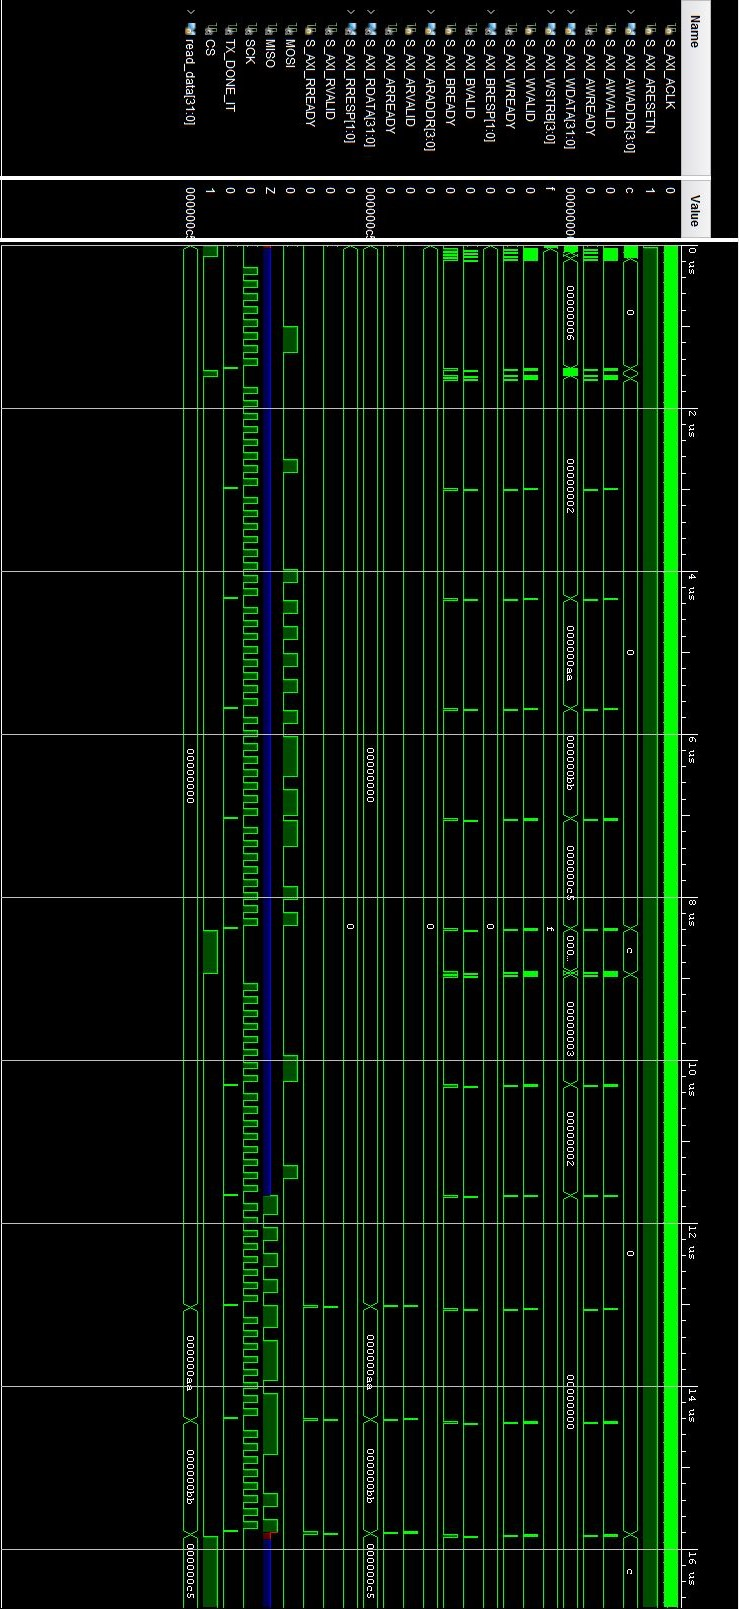
\includegraphics[scale=0.6]{sim_complete.JPG}
	\caption{A teljes szimuláció}
	\label{fig:sim_complete}
	\end{center}
\end{figure}

Az \ref{fig:sim_complete} sorszámú ábrán ábrán látható a teljes szimuláció eredménye. Láthatóak az AXI periféria írások és olvasások, illetve az SPI ciklusok. A beírt 3 adatbájt olvasáskor megjelenik a kimeneten, ebből látható hogy az SPI illesztő és az EEPROM is megfelelően működik. Ezeken felül a Vivado lehetőséget ad hogy a belső regiszterek állását is ellenőrizni lehessen, ha ezt megtesszük látható lesz hogy az EEPROM-nak valóban beíródott a belső regisztereibe az adat.

\begin{figure}[H]
	\begin{center}
	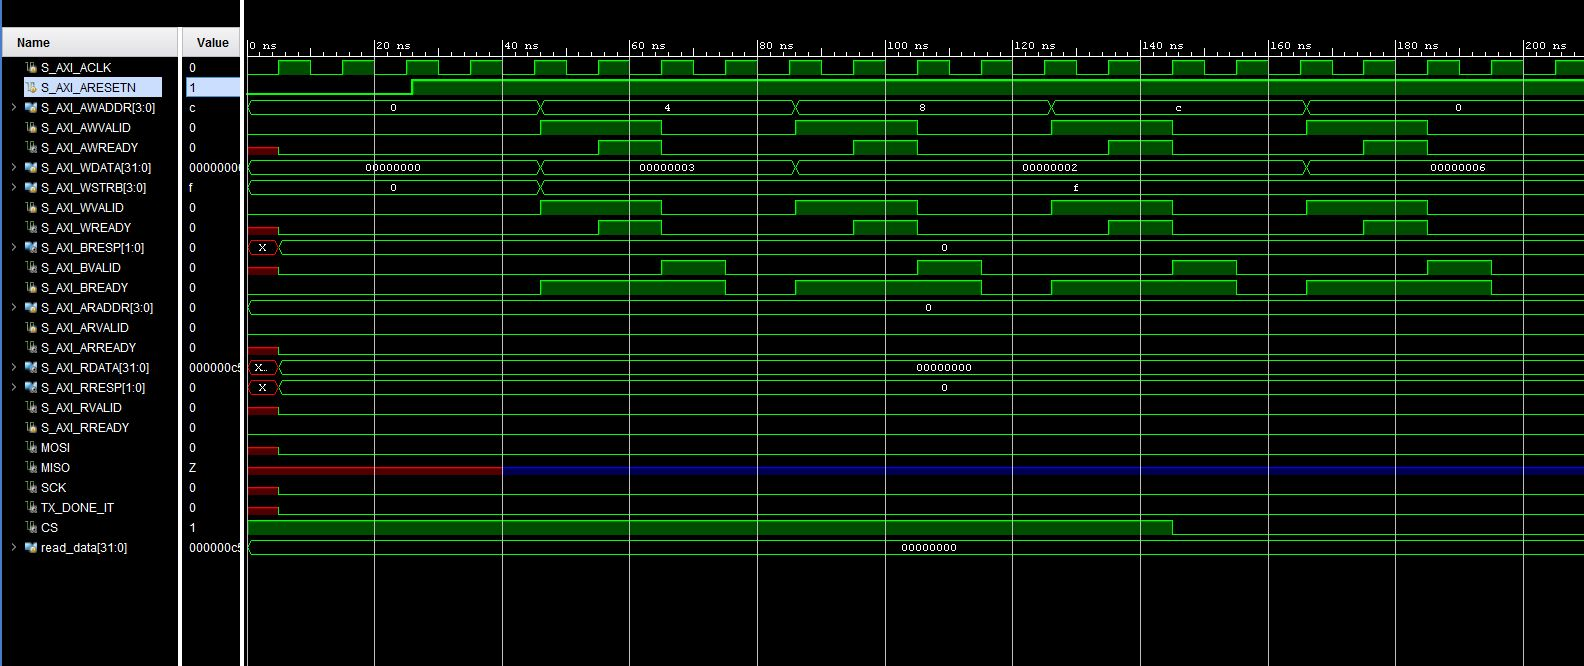
\includegraphics[scale=0.5]{axi_write.JPG}
	\caption{AXI írási ciklusok}	
	\label{fig:axi_write}
	\end{center}
\end{figure}

A \ref{fig:axi_write} sorszámú ábrán látható egy AXI írási ciklus. Látható hogy a cím és adatcsatorna egyszerre működtethető, mindkettő jelzi hogy új adat érkezik, majd vár a slave felől a válasz jelre hogy a handshake megtörténjen és az adat beíródjon a slave eszközbe. Az írásra a slave eszköz a write-response csatornán választ ad a megfelelő hibakóddal (esetünkben csak 0 lehet) és ezzel a master befejezi az írási ciklust. Mivel az AXI Lite nem támogat burst átvitelt így itt minden adatot egy komplett írási ciklussal kell átvinni.

\begin{figure}[H]
	\begin{center}
	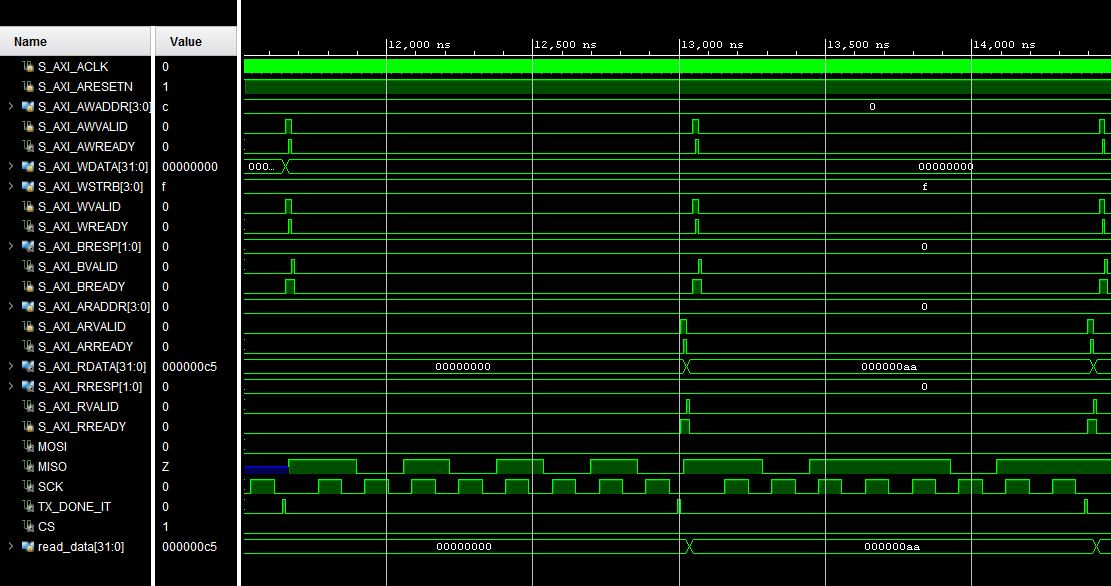
\includegraphics[scale=0.7]{SPI.JPG}	
	\end{center}
	\caption{SPI kommunikáció}
	\label{fig:spisim}
\end{figure}

Maga az SPI működése a \ref{fig:SPI} sorszámú ábrán látható. Látszik hogy a feladatban megadott üzemmód szerint felfutó SCK jelre történik az adat mintavételezése, míg lefutó élre az új adat kiküldése. Látszik hogy amíg az EEPROM-nak nem küldünk írási utasítást a kimenete (MISO) magas impedanciás állapotban van. Látható hogy a TXCOMPLETE interrupt minden tranzakció végén egy óralejre megjelenik, ezzel jelezve a ciklus befejeződését. Érdekes megfigyelni hogy mivel az EEPROM valós időzítésekkel szimulál, az új adatot csak az SCK lefutása után jelentős idővel küldi ki.

\begin{figure}[H]
	\begin{center}
	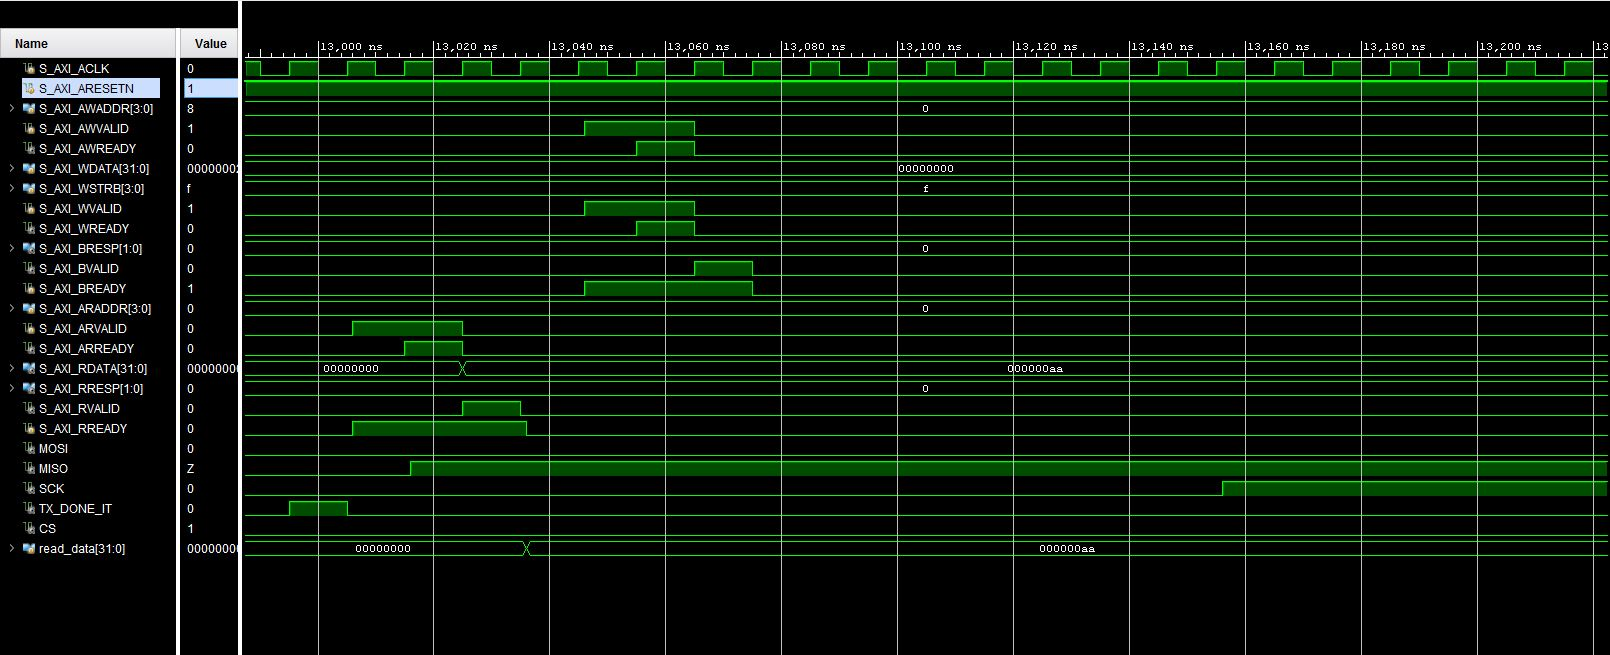
\includegraphics[scale=0.49]{axi_read.JPG}
	\caption{AXI olvasási ciklusok}
	\label{fig:axi_read}
	\end{center}
	
\end{figure}

A \ref{fig:axi_read} látható egy AXI olvasási ciklus. Látszik hogy a címet megadva és a handshake után megjelenik a kiolvasandó adat a megfelelő csatornáján.

\section{Forráskód}

\subsection{SPI}

\lstinputlisting[
language=Verilog,
inputencoding=latin1,
basicstyle=\fontsize{7}{13}\selectfont\ttfamily,
keywordstyle=\color{blue}\ttfamily,
commentstyle=\color{OliveGreen}\ttfamily,
backgroundcolor = \color{lightgray}
]{../spi_master/spi_master.srcs/sources_1/new/SPI_MASTER.v}

\subsection{Busz illesztő}

\lstinputlisting[
language=Verilog,
inputencoding=latin1,
basicstyle=\fontsize{7}{13}\selectfont\ttfamily,
keywordstyle=\color{blue}\ttfamily,
commentstyle=\color{OliveGreen}\ttfamily,
backgroundcolor = \color{lightgray}
]{../spi_master/spi_master.srcs/sources_1/new/AXI_LITE_CNTRL.v}

\subsection{Szimulációs kód}

\lstinputlisting[
language=Verilog,
inputencoding=latin1,
basicstyle=\fontsize{7}{13}\selectfont\ttfamily,
keywordstyle=\color{blue}\ttfamily,
commentstyle=\color{OliveGreen}\ttfamily,
backgroundcolor = \color{lightgray}
]{../spi_master/spi_master.srcs/sim_1/new/EEPROM_SPI_TB.v}

\pagebreak
\begin{thebibliography}{}

\bibitem{name1}

\textit{SPI leírása}
\url{https://en.wikipedia.org/wiki/Serial_Peripheral_Interface_Bus}

\today

\bibitem{name2}

\textit{AXI Lite leírása és időzítési diagramja}\\
\url{https://www.xilinx.com/support/documentation/ip_documentation/axi_lite_ipif/v3_0/pg155-axi-lite-ipif.pdf}

\today

\bibitem{name3}

\textit{EEPROM leírása}\\
\url{http://ww1.microchip.com/downloads/en/DeviceDoc/21832H.pdf}

\today

\bibitem{name4}

\textit{}\\
\url{}
\today

\bibitem{name5}

\textit{}\\


\bibitem{name6}

\textit{}\\
\url{}
\today


\end{thebibliography}
\end{document}
